\documentclass[conference]{IEEEtran}
\IEEEoverridecommandlockouts
% The preceding line is only needed to identify funding in the first footnote. If that is unneeded, please comment it out.
\usepackage{cite}
\usepackage{amsmath,amssymb,amsfonts}
\usepackage{algorithmic}
\usepackage{graphicx}
\usepackage{textcomp}
\usepackage{xcolor}
\usepackage{booktabs}
\usepackage{tabularx}
\usepackage{hyperref}
\def\BibTeX{{\rm B\kern-.05em{\sc i\kern-.025em b}\kern-.08em
    T\kern-.1667em\lower.7ex\hbox{E}\kern-.125emX}}
\begin{document}

\title{Real-time Domain Adaptation in Semantic Segmentation\\
{\footnotesize \textsuperscript{}}
}

\author{\IEEEauthorblockN{1\textsuperscript{st} Berardo Nicholas}
\IEEEauthorblockA{\textit{dept. Computer Engineering} \\
\textit{Politecnico di Torino}\\
Turin, Italy \\
s319349@studenti.polito.it}
\and
\IEEEauthorblockN{2\textsuperscript{nd} Cardona Riccardo}
\IEEEauthorblockA{\textit{dept. Computer Engineering} \\
\textit{Politecnico di Torino}\\
Turin, Italy \\
s319441@studenti.polito.it}
\and
\IEEEauthorblockN{3\textsuperscript{rd} De Marco Alessando}
\IEEEauthorblockA{\textit{dept. Computer Engineering} \\
\textit{Politecnico di Torino}\\
Turin, Italy \\
s317626@studenti.polito.it}
}

\maketitle

\begin{abstract}
%We use an efficient structure named Short-Term Dense Concatenate network (STDC network) for the semantic segmentation task. This structure reduces the dimension of feature maps and uses the aggregation of them for image representation, then uses a Detail aggregation module for producing the low-level features. Finally, these two are merged to produce the segmentation result. We test this model on
%Cityscapes and GTA V, following the evaluation of the domain shift between GTA V and Cityscapes and the implementation of an unsupervised adversarial domain adaptation method used for reducing the domain shift. Finally, we provide also a way to make the discriminator of the domain adaptation method faster and lighter. Results are also shown for all the experiments we did. We express the mean Intersection over Union (mIoU) and Precision and train time per epoch of each experiment.
Semantic segmentation, a core task in computer vision, requires high accuracy and real-time performance for applications in autonomous driving and urban scene understanding. However, the domain shift between training datasets (e.g., synthetic images) and real-world scenarios poses a significant challenge, necessitating effective domain adaptation techniques. This paper introduces an approach to real-time domain adaptation in semantic segmentation utilizing the Short-Term Dense Concatenate network (STDC) model, a variant of BiSeNet optimized for speed and efficiency. We target the adaptation from a synthetic domain, specifically the GTA5 dataset, to real-world urban scenes, represented by the Cityscapes dataset. Our methodology employs adversarial learning as the pivotal mechanism for domain adaptation. Initially, we utilize a classical discriminator with five convolutional layers to align feature distributions between the source and target domains. To enhance efficiency and reduce computational demands, we then explore an innovative discriminator architecture incorporating depthwise separable convolutional layers, aiming for a lightweight and faster adaptation process without compromising accuracy. Experimental results demonstrate the effectiveness of our approach, showcasing improvements in segmentation performance on the Cityscapes dataset while maintaining real-time processing capabilities.
\end{abstract}





\section{Introduction}
Semantic Segmentation is a pivotal area within computer vision, tasked with assigning a unique label to each pixel in an image. This technology is used in various applications, including autonomous vehicles, video surveillance and robot sensing, due to its ability to provide detailed contextual information about environmental elements. While numerous models have achieved commendable accuracy in semantic segmentation, the quest for real-time processing often necessitates the adoption of lightweight neural architectures. Such a choice, however, frequently entails a significant compromise on accuracy due to reduced model complexity.
In response to these challenges, some new methods were investigated, such as feature fusion and aggregation modules. Additionally, some approaches involve downsizing the input image resolution, which, while beneficial for computational efficiency, can adversely affect the model's ability to accurately delineate boundaries and recognize smaller objects.

The main problem in semantic segmentation remains the procurement of accurately annotated datasets. High-quality annotations, requiring pixel-level precision, are tedious and costly to produce, making fully annotated datasets a rarity. To mitigate this, synthetic datasets, such as GTAV, have been introduced, offering comprehensive or partially annotated images that necessitate minimal human intervention. This dataset can be used to train jointly with a real-world dataset or alone, but training on a synthetic dataset alone can result in a generalization problem, when testing it on a real-world dataset. This is caused mainly due to the domain shift between the source and target dataset. Although we can try to generate a synthetic dataset that looks like real-world data to reduce the domain shift, it is necessary to apply some domain adaptation between the two datasets.
\begin{figure}[!t]
\centering
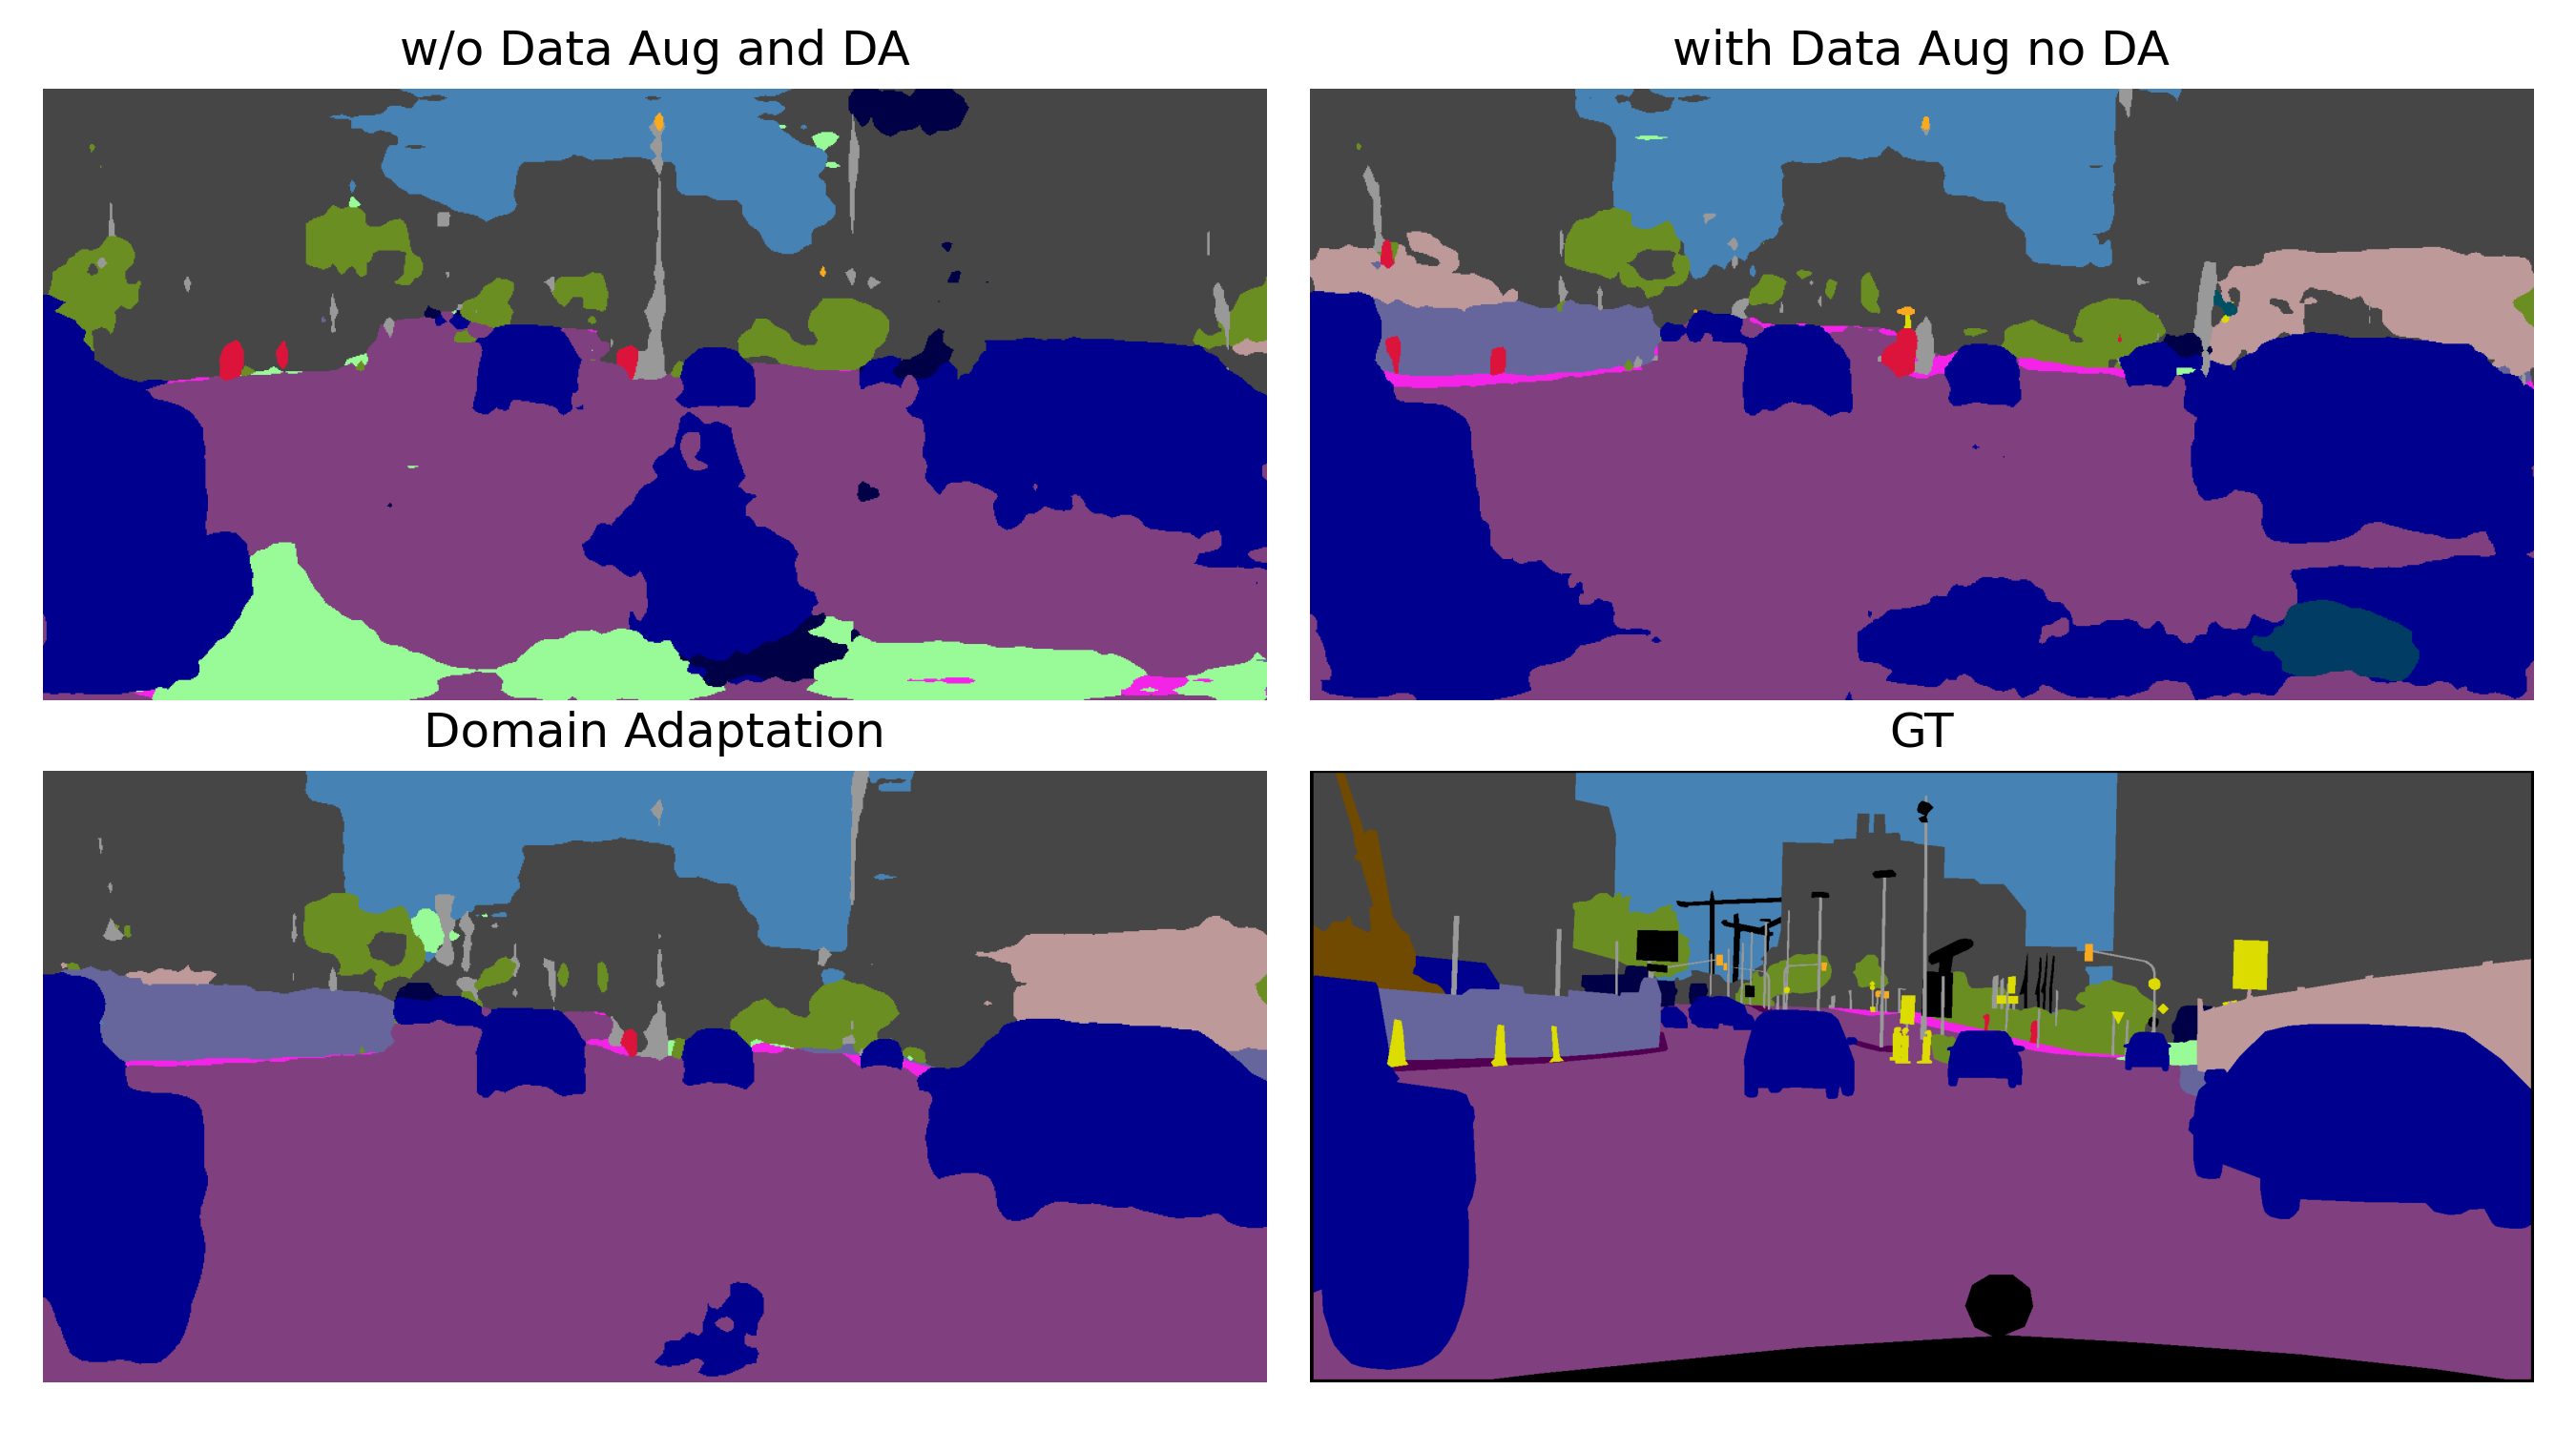
\includegraphics[width=\linewidth]{figures/small.png}
\caption{Segmentation results illustrating the impact of data augmentation (Data Aug) and domain adaptation (DA) techniques on a Cityscapes image.}
\end{figure}

The Short-Term Dense Concatenate network (STDC net) \cite{b1} represents a paradigm shift towards lightweight, efficient models in semantic segmentation. As depicted in Figure ~\ref{fig:stdc_net}, STDC net employs a multi-scale encoding strategy, with a deliberate reduction in kernel size to expedite computation, balancing performance with an acceptable compromise in accuracy. Starting from BiSeNet \cite{b2}, which bifurcates into a Spatial Path for preserving spatial features of the original image, and a Context Path for capturing contextual information, STDC network is used as the backbone of the Context Path. Attention Refine Module (ARM) is used in the Context Path to refine some features and Future Fusion Model (FFM) is used to fuse the output of the Spacial Path with the output of the Context Path.

Domain adaptation emerges as a critical step in addressing the performance degradation encountered when models trained on specific datasets are applied to previously unseen data. This degradation is primarily attributed to the domain shift between the training (source) and testing (target) datasets, manifesting in variations across cities, weather conditions, and lighting. Domain adaptation methods are used to close the gap between source and target domains. In this paper, we adopt an adversarial domain adaptation method \cite{b3} composed of a segmentation model to predict the output and a discriminator to predict if the input is from the source or target domain. The objective is to produce segmentation results indistinguishable from the discriminator, signifying alignment between source and target domain outputs. Our experiments focus on the adaptation from the synthetic GTAV \cite{b4} dataset to the real-world Cityscapes \cite{b5} dataset, illustrating the domain shift challenge and our method's effectiveness in smalling this gap.

The final step is making the discriminator lighter and faster. Taking inspiration from MobileNets \cite{b6}, depthwise separable convolutions are adopted, where each block is composed of a depthwise convolution that filters each input channel and a pointwise convolution that combines the output of the depthwise convolution with a 1 x 1 kernel. The depthwise convolution takes the receptive field of \(D_K\) kernel size but for only one feature and the pointwise convolution looks at the entire feature, but with a 1 x 1 kernel size. Combining them we obtain an output with a \(K_D\) receptive field over all features, that is the same thing obtained by the standard convolution layer.

Our contributions can be summarized as follows:
%First, we build the STDC network and train it on Cityscapes and test it again on Cityscapes. Second, we reply the same idea over the GTAV dataset, so train on GTAV and test on GTAV. Third, we compute the domain shift between GTAV (source) and Cityscapes (target) domains firstly in vanilla, then with some augmentation on GTAV. Fourth, we implement the adversarial domain adaptation method and test it with GTAV as the source domain and Cityscapes as the target domain. Lastly, we apply some real-time semantic segmentation methods to our discriminator function to make it faster.
\begin{enumerate}
    \item We demonstrate the STDC network's efficacy on the Cityscapes dataset, both in the training and testing phases.
    \item We replicate this methodology with the GTAV dataset to evaluate performance within synthetic environments.
    \item We quantify the domain shift between GTAV (source) and Cityscapes (target), initially under standard conditions and subsequently with augmented GTAV data.
    \item We implement an adversarial domain adaptation technique, assessing its performance in harmonizing the GTAV and Cityscapes datasets.
    \item Lastly, we incorporate convolutional depthwise separable into our discriminator, improving its speed and efficiency.
\end{enumerate}

Here a look to our implementation: \url{https://github.com/Riden15/Real-time-Domain-Adaptation-in-Semantic-Segmentation}

\begin{figure}[t]
\centerline{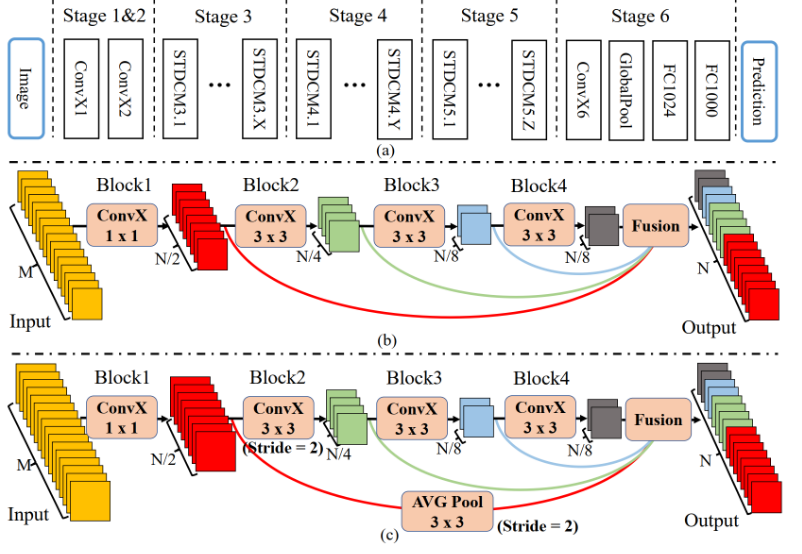
\includegraphics[width=0.4\textwidth]{figures/Figure1-STDCnet}}
\caption{STDC network.}
\label{fig:stdc_net}
\end{figure}

\section{Related Work}

\subsection{Real-Time Semantic Segmentation}
Real-time semantic segmentation demands algorithms that not only deliver high-quality predictions but also operate at speeds conducive to real-time processing. Several strategies have been adopted to achieve this balance, primarily through the use of lightweight model architectures. E-Net \cite{b7} exemplifies this approach by designing a model from the ground up to be both lightweight and fast, thus enabling rapid segmentation. DFANet \cite{b8} further contributes to this paradigm by leveraging a lightweight backbone to diminish computational costs significantly. BiSeNet \cite{b2} introduces a dual-path architecture, segregating the extraction of low-level details from high-level semantic information, subsequently merging them for comprehensive feature representation. In our work, we incorporate the Short-Term Dense Concatenation (STDC) backbone within the Context Path of BiSeNet, aiming to enhance real-time segmentation efficiency.

\subsection{Domain Adaptation}
Domain adaptation techniques are crucial for mitigating the domain shift encountered when applying a model trained on one dataset (source) to another (target) dataset. Such shifts can significantly degrade model performance, even when the datasets pertain to similar environments but differ in aspects like weather conditions, lighting, or camera perspectives. Aligning the feature distributions between source and target datasets emerges as a primary solution to this challenge. The Domain-Adversarial Neural Network (DANN) \cite{b9} represents a seminal approach in this direction, effectively minimizing domain discrepancies.

\section{Methods}

We first introduce the Short-Term Dense Concatenate network (STDC network) and how we used it with BiSeNet \cite{b2}, then the unsupervised adversarial domain adaptation method.

\subsection{Short-Term Dense Concatenate Network}

The STDC network, illustrated in Fig.~\ref{fig:stdc_net} (a), incorporates the innovative Short-Term Dense Concatenate Module (STDCM) at stages 3, 4, and 5, each comprising a series of ConvX blocks as shown in Fig.~\ref{fig:stdc_net} (b) and (c). For each module, the computation follows:
\begin{equation}
x_i = ConvX_i(x_{i-1}, k_i)
\end{equation}
where $x_i$ represents the output from the $i$-th ConvX block, $x_{i-1}$ is the input to the $i$-th ConvX block, and $k_i$ denotes the kernel size. Each ConvX block consists of a convolution layer, a batch normalization layer, and a ReLU activation layer. The kernel size $k_i$ is initially set to $1 \times 1$ for the first block, transitioning to $3 \times 3$ for subsequent blocks. The feature dimension is halved at each $ConvX_i$ block, $N/2^i$, maintaining the dimension for the final block, where $N$ is the total number of output channels.

As depicted in Fig.~\ref{fig:stdc_net}(c), downsampling is executed exclusively in the second block of each module. The outputs from all ConvX blocks within a module are then concatenated:
\begin{equation}
x_{output} = F(x_1, x_2, \dots, x_n)
\end{equation}
Here, $x_{output}$ denotes the module's output, $F$ represents the concatenation operation, and $x_1, x_2, \dots, x_n$ are the outputs from each ConvX block. Prior to concatenation, the feature maps are subjected to average pooling with a $3 \times 3$ kernel to ensure uniformity in spatial dimensions. Our STDC implementation comprises 4 ConvX blocks per module.

The complete STDC network, as illustrated in Fig.~\ref{fig:stdc_net}(a), spans six stages. The initial two stages consist solely of ConvX blocks. Stages 3, 4, and 5 incorporate two STDC modules each, with the first module in each stage employing a stride of 2 for downsampling, while subsequent modules maintain the spatial resolution. The final stage (Stage 6) outputs the prediction logits through a sequence of a ConvX block, global average pooling, and two fully connected layers.

\begin{figure}[tp]
\centerline{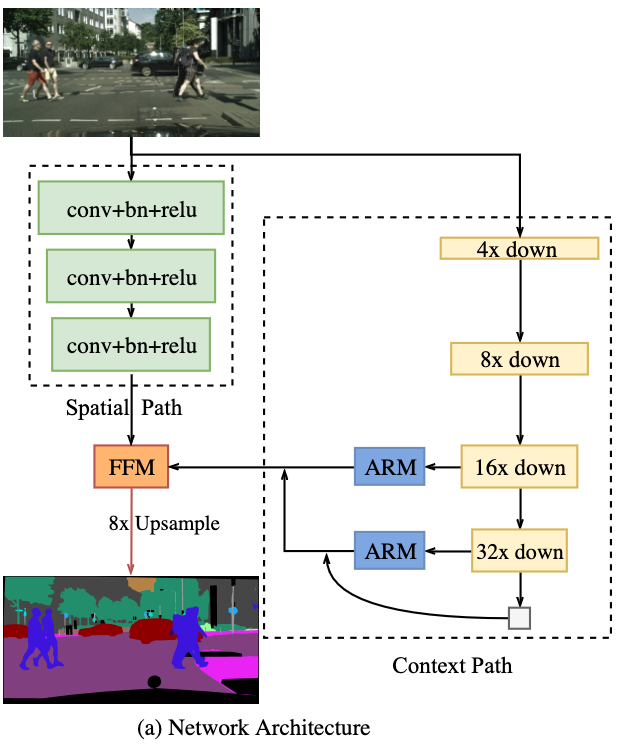
\includegraphics[width=0.4\textwidth]{figures/BiSeNet}}
\caption{BiSeNet network.}
\label{fig:bisenet}
\end{figure}

\subsection{BiSeNet}

The BiSeNet architecture, as depicted in Fig.~\ref{fig:bisenet}, strategically divides into two primary components: the Spatial Path and the Context Path, each serving a unique purpose in enhancing semantic segmentation performance.

\textbf{Spacial Path}

The Spatial Path is designed to tackle the common trade-off between performance and spatial detail retention in real-time semantic segmentation. While some models opt for reduced input image sizes to improve computational efficiency, this often results in a significant loss of spatial detail, adversely affecting segmentation accuracy. Similarly, lightweight models achieve speed at the cost of detailed spatial information due to channel pruning. Contrarily, BiSeNet's Spatial Path consists of three sequential blocks, each featuring a convolution operation with a stride of 2, followed by batch normalization and ReLU activation \cite{b9}. This configuration effectively downsamples the original image to 1/8 of its size while preserving critical spatial information, a key factor in maintaining high segmentation accuracy.

\textbf{Context Path}

The Context Path employs the STDC network as its backbone, particularly leveraging stages 3, 4, and 5 to diminish the feature map size, thereby expanding the receptive field crucial for capturing context. Incorporation of a global average pooling layer at the Context Path's conclusion further aids in this expansion. Attention Refine Modules (ARM) are integrated within stages 4 and 5 to refine the feature maps, ensuring that only the most relevant contextual information is forwarded through the network. The culminating step involves the Feature Fusion Module (FFM), which synergistically combines the detailed 1/8 scale features from the Spatial Path with the context-enriched features from the Context Path. This dual-path strategy ensures that the final segmentation output benefits from both detailed spatial information and a broad contextual understanding, pivotal for achieving accurate and real-time semantic segmentation.

\textbf{Attention Refine Module}
\begin{figure}[tp]
\centerline{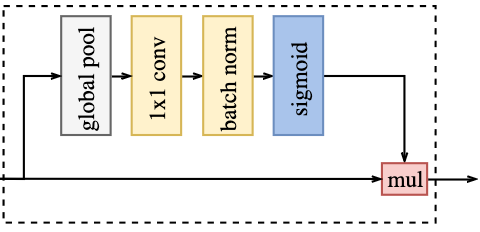
\includegraphics[width=0.4\textwidth]{figures/ARM}}
\caption{Attention Refine Module}
\label{fig:arm}
\end{figure}

The Attention Refine Module (ARM) is a pivotal component within the Context Path, enhancing the feature refinement process for the latter stages of the network. As depicted in Fig.~\ref{fig:arm}, ARM employs a global average pooling mechanism to encapsulate global contextual cues, subsequently generating an attention vector. This vector acts as a guide for feature refinement, enabling more precise and contextually informed feature learning.

\textbf{Future Fusion Model}

The Feature Fusion Model (FFM), as illustrated in Fig.~\ref{fig:ffm}, plays a critical role in integrating the outputs of the Context Path, facilitated by the STDC network, with those from the Spatial Path. A significant challenge in this integration is reconciling the disparate levels of representation between the two paths—the Context Path encodes contextual information, whereas the Spatial Path captures spatial details. Direct summation of these outputs is insufficient due to their qualitative differences in representation. FFM addresses this challenge by effectively merging these distinct feature sets, ensuring a harmonious blend of spatial and contextual information, crucial for accurate semantic segmentation.

\begin{figure}[tp]
\centerline{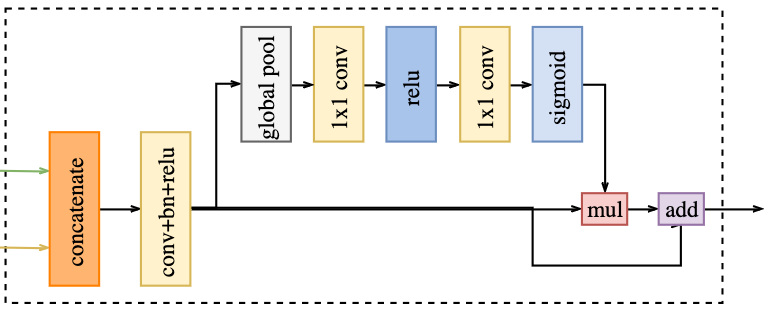
\includegraphics[width=0.4\textwidth]{figures/FFM}}
\caption{Future Fusion Model}
\label{fig:ffm}
\end{figure}

\subsection{Adversarial Domain Adaptation}

At the core of our unsupervised adversarial domain adaptation approach \cite{b3} lies the objective to train a segmentation network capable of classifying images from both the source domain (with labels) and the target domain (without annotations). This process involves generating predictions for images from both domains and subsequently feeding these predictions to a discriminator. The discriminator's task is to ascertain the domain of origin for each input. A key component of this methodology is a loss function that incentivizes the segmentation network to produce indistinguishable predictions for the two domains. We utilize the BiSeNet architecture, as elaborated in previous sections, as our segmentation network. The domain adaptation loss function is formulated as follows:
\begin{equation}
L(I_s,I_t) = L_{seg}(I_s) + \lambda_{adv} \cdot L_{adv}(I_t)
\end{equation}
where $L_{seg}$ denotes the cross-entropy loss for source domain predictions, $\lambda_{adv}$ is a weighting factor to balance the adversarial loss $L_{adv}$, which is implemented using BCEWithLogitLoss.

The procedure begins by forwarding the source image $I_s$ through the segmentation network to obtain its prediction $P_s$ and calculating $L_{seg}$ using $I_s$'s label. Subsequently, the target image $I_t$ is processed to generate the prediction $P_t$, which is fed into the discriminator to compute $L_{adv}$. This loss is then used to optimize the segmentation network. The optimization of the discriminator involves calculating the loss for images from the GTAV dataset (labeled as 1) and the Cityscapes dataset (labeled as 0), sequentially.

The discriminator's architecture is characterized by five convolutional layers with a kernel size of $4 \times 4$ and a stride of 2. The number of channels across these layers is sequentially \{64, 128, 256, 512, 1\}. Each convolutional layer, except for the last, is succeeded by a leaky ReLU activation function \cite{b9} with a coefficient of 0.2. To match the input size, an up-sampling layer follows the final convolutional layer, resizing the discriminator's output accordingly.

\subsection{Depthwise Separable Convolution}

\begin{figure}[tp]
\centerline{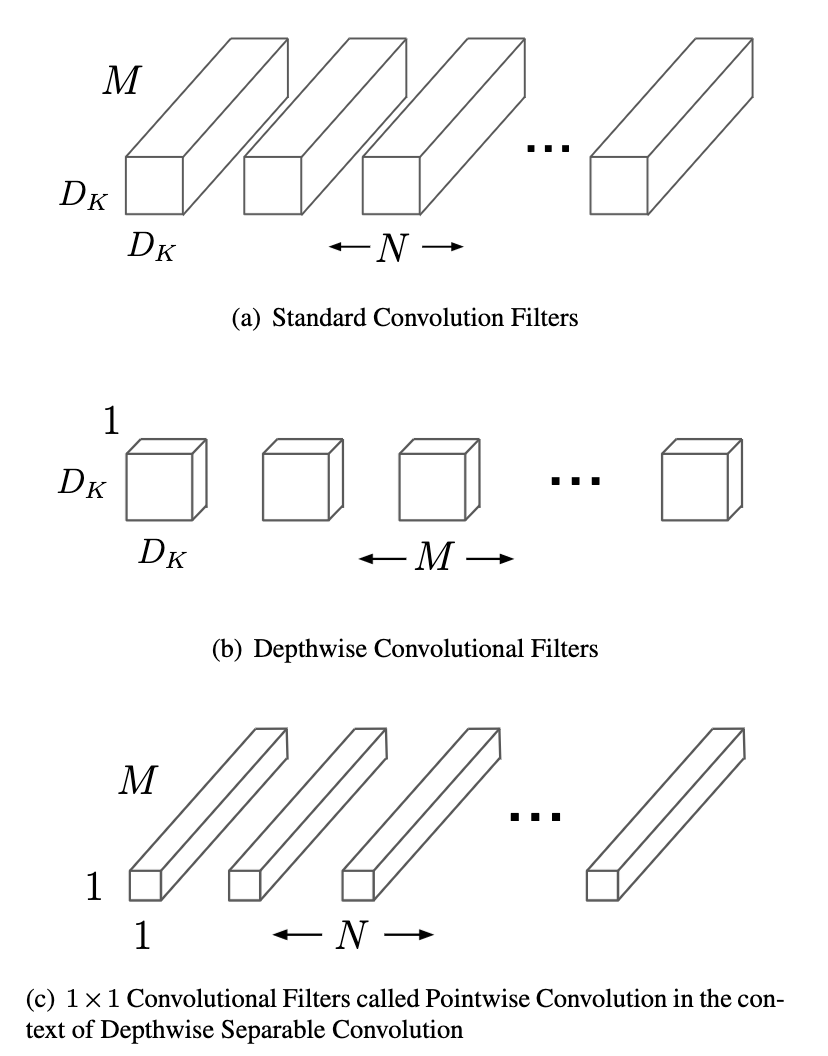
\includegraphics[width=0.4\textwidth]{figures/depthwise ocnv.pdf.png}}
\caption{Depthwise separable convolution. The standard convolutional filters in (a) are replaced by two layers: depthwise convolution in (b) and pointwise convolution in (c) to build a depthwise separable filter}
\label{fig:depthwise}
\end{figure}

To enhance the efficiency and speed of our discriminator, we adopted depthwise separable convolutions, inspired by the MobileNets architecture \cite{b6}. This approach decomposes a standard convolution into two distinct layers: depthwise and pointwise convolutions, as depicted in Fig.~\ref{fig:depthwise}.

\textbf{Depthwise convolutions} operate by applying a single filter per input channel, effectively isolating the filtering process to individual channels.

\textbf{Pointwise convolutions}, following depthwise convolution, employ a $1 \times 1$ convolution to amalgamate the filtered outputs across all channels.

This bifurcation of the convolution process enables a significant reduction in computational complexity. The standard convolution, which simultaneously filters and combines inputs across channels, is replaced by a two-step process: depthwise convolution for filtering, followed by pointwise convolution for combining these filters, as illustrated in Fig.~\ref{fig:depthwise}. The resultant architecture maintains the receptive field and feature richness of a standard convolution while substantially decreasing the computational load.

Our discriminator leverages blocks consisting of a depthwise convolution layer, a leaky ReLU activation \cite{b9}, a pointwise convolution layer, and another leaky ReLU, streamlining the model for real-time applications.

\subsection{Diagonalwise Refactorization with Grouping Mechanism}
In our experimentation, we adopted the Diagonalwise Refactorization technique \cite{b10}, an innovative approach designed to enhance the computational efficiency of depthwise separable convolution layers. This method should improves GPU utilization by reorganizing the convolutional filters into a large diagonal matrix, where each filter is aligned diagonally and all other elements are set to zero. This restructuring allows for leveraging the high-performance computing capabilities of GPUs more effectively by transforming depthwise convolutions into an equivalent standard convolution operation, which can be accelerated using optimized libraries such as Pytorch.

To further optimize the computational process, especially in scenarios involving a high number of input channels, following \cite{b10}, we implemented a grouping mechanism. This technique entails dividing the input channels into several groups, with each group undergoing Diagonalwise Refactorization independently. Specifically, for a convolution layer with $M$ input channels, we divide these channels into $G$ groups, each containing $M/G$ channels. This division enables parallel processing of smaller, more manageable convolution operations, thus reducing computational complexity and enhancing parallelism on the GPU.

The grouping mechanism is dynamically adjusted based on the total number of input channels, ensuring scalability and flexibility across different network architectures and hardware configurations.

\subsection{Discriminator Architecture Comparison}

To underscore the efficiency gains from integrating advanced convolution techniques in our discriminator, we present an architectural comparison featuring traditional, depthwise separable, and diagonalwise refactorization approaches:


\begin{table}[h]
\centering
\caption{Comparison of discriminator architectures: Classic vs. Depthwise Separable vs Diagonal Depthwise. Input size (8, 19, 1024, 512)}
\label{tab:discriminator_comparison}
\begin{tabular}{lcc}
\hline
\textbf{Architecture} & \textbf{Total Parameters} & \textbf{Total Mult-Adds (GB)} \\
\hline
Classic & 2,781,121 & 123.64 \\
Depthwise Separable & 191,364 & 8.72 \\
Diagonalwise & 1,168,352 & 7.72 \\
\hline
\end{tabular}
\end{table}

The inclusion of depthwise separable and diagonalwise refactorization in the discriminator architecture demonstrates substantial efficiency improvements over the classic architecture. The depthwise separable configuration offers a significant reduction in both the total number of parameters and computational complexity, as measured by total multiply-add operations (Mult-Adds). The diagonalwise refactorization further enhances this efficiency, achieving a lower total of Mult-Adds, indicative of its optimized computational footprint. These advancements highlight the potential of employing sophisticated convolutional strategies for real-time semantic segmentation tasks, enabling faster processing and reduced resource consumption without compromising the model's performance.

\section{Experiments}

We conducted a series of experiments to evaluate the performance of the STDC network across various settings and domain adaptation strategies. These experiments were designed to assess the effectiveness of our model under different conditions, including training and testing on identical datasets, as well as cross-dataset evaluations to gauge domain adaptation performance.

\begin{table*}[]
\centering
\caption{Experiments. The dataset on the left of the arrow is the source dataset, and the one on the right is the target dataset. For each test we measure the Accuracy, the mean Intersection over Union and the average train time per epoch. The second and third have the same train time because the model used in the third is the same one used in the second, only the test dataset changes}
\label{TrainingTimeAndAccuracy}
\begin{tabularx}{\textwidth}{@{}Xccc@{}}
\toprule
& Accuracy (\%) & mIoU (\%) & Train time (avg per-epoch) \\ \midrule
Cityscapes $\rightarrow$ Cityscapes & 81.1 & 57.8 & 2:33 minutes \\
GTA V $\rightarrow$ GTA V & 80.8 & 62 & 3:28 minutes \\
GTA V $\rightarrow$ Cityscapes w/o Data Augmentation & 60.1 & 24.6 & 3:28 minutes \\
GTA V $\rightarrow$ Cityscapes w Data Augmentation & 70.2 & 30.7 & 5:22 minutes \\
GTA V $\rightarrow$ CityScapes w Domain Adaptation & 74.3 & 33.8 & 4:33 minutes \\
GTA V $\rightarrow$ CityScapes w Depthwise Separable Discriminator & 73.1 & 32.7 & 4:32 minutes \\
GTA V $\rightarrow$ CityScapes w Diagonal Depthwise Discriminator & 74.0 & 33.5 & 4:25 minutes \\
\bottomrule
\end{tabularx}
\end{table*}


\begin{figure}[tp]
\centerline{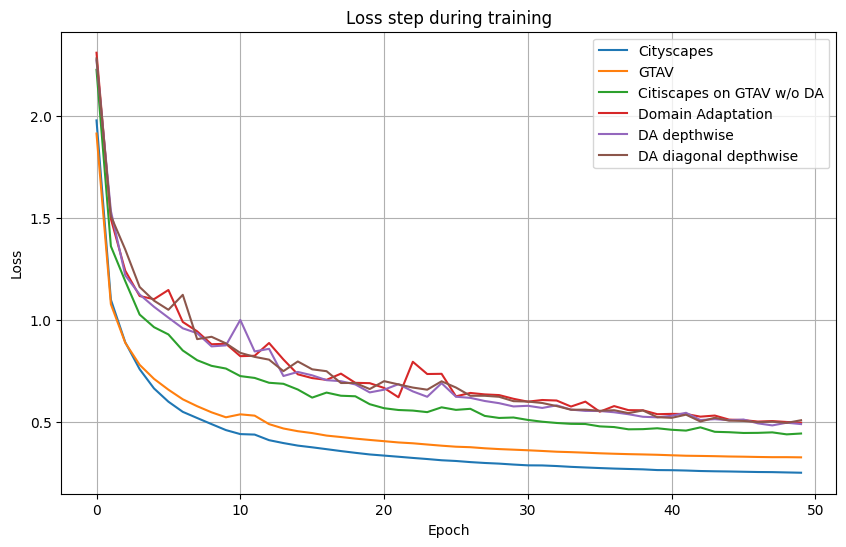
\includegraphics[width=0.4\textwidth]{figures/loss}}
\caption{Loss step during training. On the X we have the epochs, on Y we have the loss.}
\label{fig:loss_steps}
\end{figure}

\begin{figure}[tp]
\centerline{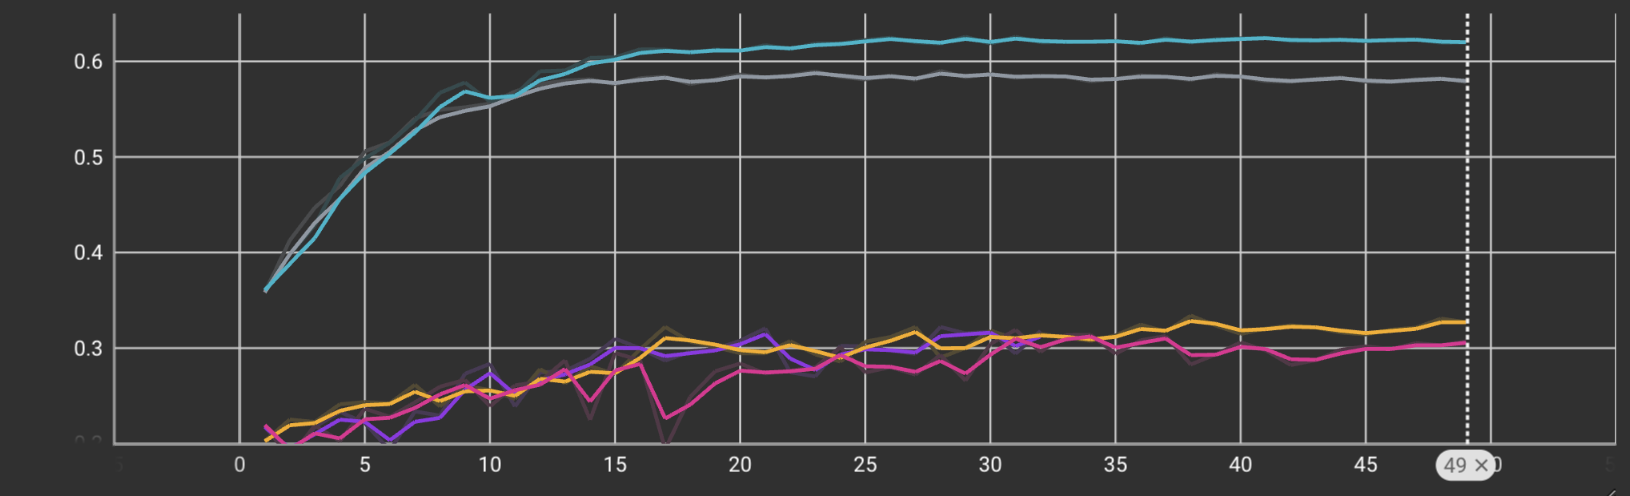
\includegraphics[width=0.4\textwidth]{figures/miou}}
\caption{mIoU during training. On the X we have the epochs, on Y we have the mIoU.}
\label{fig:miou}
\end{figure}

\begin{figure}[tp]
\centerline{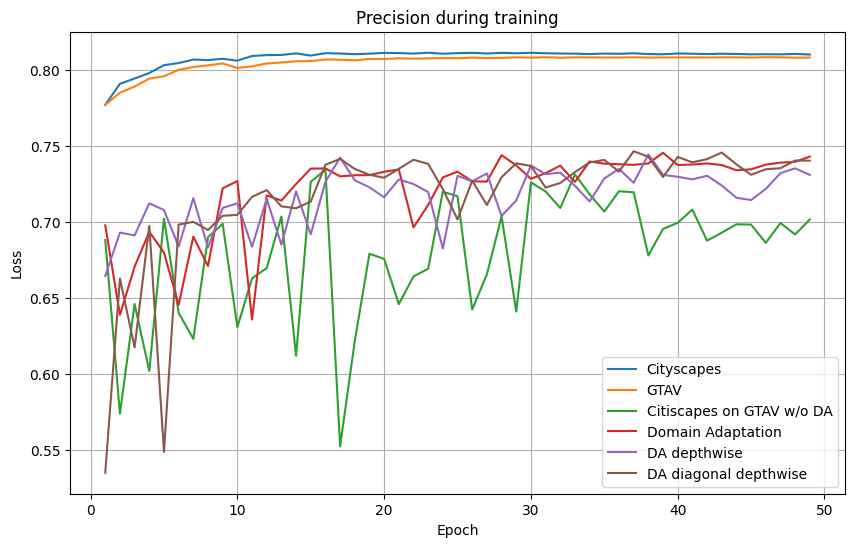
\includegraphics[width=0.4\textwidth]{figures/precision}}
\caption{Precision during training. On the X we have the epochs, on Y we have the precision.}
\label{fig:precision}
\end{figure}

\subsection{GTA5 Dataset}
The GTA5 dataset \cite{b4}, synthesizing approximately 2.500 images from the video game set in a virtual Los Angeles, offers a high-resolution format of 1914 x 1052 pixels. Accompanied by ground truth annotations for semantic segmentation, the dataset aligns with 19 semantic categories, mirroring those used in the Cityscapes dataset to ensure compatibility between the two. Initially, the GTA5 dataset serves to evaluate our model in isolation, where training and testing phases are conducted exclusively within this synthetic environment. Subsequently, it is employed as the source domain in our domain adaptation experiments.

\subsection{Cityscapes Dataset}
The Cityscapes dataset \cite{b5} comprises approximately 2.000 finely annotated images, divided into sets for training (1.568 images), validation (500 images). While the dataset encompasses 30 classes, only 19 are utilized for semantic segmentation tasks, consistent with the GTA5 dataset. Original images present a very high resolution of 2048 x 1024 pixels; however, for computational efficiency, we scale them down to 1024 x 512 pixels. Similar to the GTA5 dataset, Cityscapes is first used to assess the model's performance in isolation, with subsequent employment as the target domain in our domain adaptation framework.

\begin{figure*}[htbp]
  \centering
  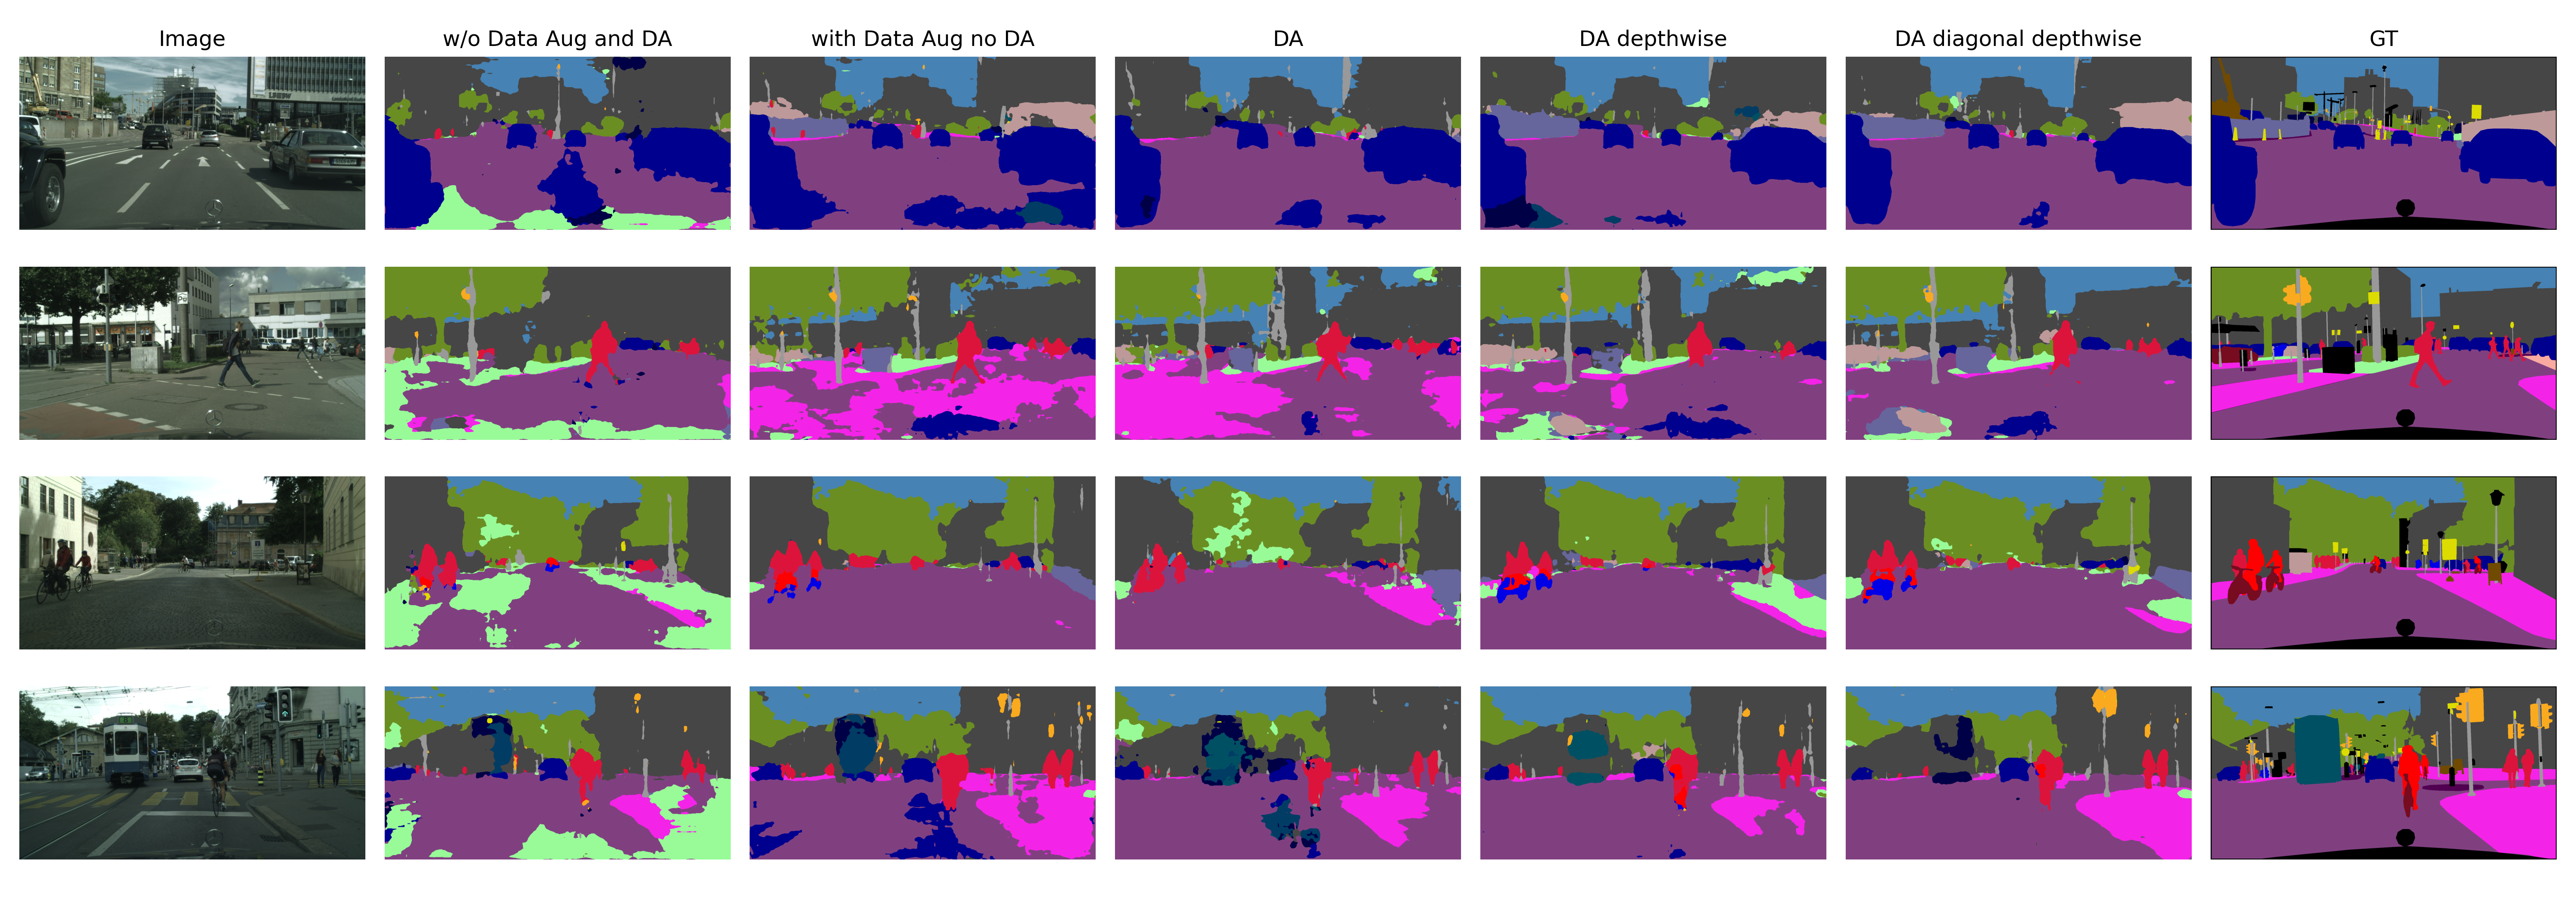
\includegraphics[width=\textwidth]{figures/all.png}
  \caption{Comparative visualization of semantic segmentation results across different models and techniques. Each row shows the original Cityscapes image with corresponding segmentation outputs. From left to right: the raw image, segmentation without data augmentation and domain adaptation (DA), with data augmentation but no DA, with DA using a classical convolutional approach, with DA employing depthwise separable convolutions, with DA utilizing diagonal depthwise separable convolutions, and the ground truth (GT) segmentation. These visual results highlight the progressive improvement in segmentation fidelity as we move from standard methods to advanced DA techniques.}
  \label{fig:all_result}
\end{figure*}


\subsection{Experimental Setup}

Our initial experiments focused on training the STDC model using:
\begin{itemize}
    \item The Cityscapes dataset, with a batch size of 8, over 50 epochs, employing SGD as the optimizer with a learning rate of 0.01.
    \item The GTA V dataset, under identical conditions to the Cityscapes training, to evaluate the model within a synthetic environment.
    \item Cross-dataset training from GTA V to Cityscapes, to understand the model's capability in adapting from synthetic to real-world imagery without and with data augmentation, maintaining the same training parameters.
\end{itemize}

Furthermore, we explored the efficacy of domain adaptation using discriminators of varying architectures:
We experimented with a classic convolutional architecture and two variants featuring depthwise separable convolutions: one utilizing a standard depthwise separable discriminator and another with diagonal depthwise separable layers. In these experiments, the optimizer settings for the segmentation network (referred to as the generator in the context of adversarial training) and the discriminator were carefully chosen to balance training stability and convergence speed. For the segmentation network, we employed Stochastic Gradient Descent (SGD) with a learning rate of 0.1, momentum of 0.9, and weight decay set to $5 \times 10^{-4}$. The discriminator was optimized using the Adam optimizer with a learning rate of 0.001. These configurations were applied consistently across all discriminator models, maintaining a batch size of 8 and spanning 50 training epochs.


\subsection{Results and Discussion}

The results of our experiments are summarized in Table \ref{TrainingTimeAndAccuracy}, accompanied by figures illustrating the loss Fig.~\ref{fig:loss_steps}, mean Intersection over Union (mIoU) Fig.~\ref{fig:miou}, and precision Fig.~\ref{fig:precision} for each experimental condition.

Implementing the depthwise separable convolution in the discriminator aimed to achieve a lighter and faster model. This adaptation resulted in a significant reduction in model parameters and computational complexity, as shown in Table \ref{tab:discriminator_comparison}, although with a slight decrease in performance compared to the classic discriminator model. Notably, no improvement in training time was observed, attributed to the current lack of optimization for depthwise separable layers on GPUs. This hypothesis was supported by further experiments across various GPU Table \ref{tab:GPUTimeDiscminator} and CPU Table \ref{tab:CPUTimeDiscminator} configurations, which indicated increased training speed on CPUs but not on GPUs, suggesting that depthwise separable layers are not yet optimized for GPU parallelization.

To address this, we introduced a discriminator with diagonal depthwise separable convolutions, expecting improved training efficiency without significantly increasing parameter count. However, the results did not meet our expectations, yielding better mIoU than the standard depthwise separable model but inferior to the classic model. Moreover, reduced training times were observed only on specific GPU models, leading to the conclusion that advancements in GPU and deep learning frameworks since 2018 have diminished the efficiency advantage of diagonal depthwise separable layers over their standard counterparts.

In conclusion, while the classic discriminator model yielded the highest mIoU scores, the diagonal depthwise separable discriminator offered the best training times on select GPUs, notably the NVIDIA RTX 4070. Overall, the standard depthwise separable model presents the best compromise between mIoU performance and training efficiency.



\begin{table}[]
\centering
\caption{Passing a tensor of size (8, 19, 1024, 512) to the Discriminator only once in the CPU}
\begin{tabular}{@{}lccc@{}}
\toprule
                                 & \begin{tabular}[c]{@{}c@{}}5800x\\ (sec)\end{tabular} & \begin{tabular}[c]{@{}c@{}}Colab CPU\\ (sec)\end{tabular} & \begin{tabular}[c]{@{}c@{}}Colab TPU\\ (sec)\end{tabular} \\ \midrule
Train Discriminator              & 0.62                                                  & 7.18                                                      & 6.20                                                      \\
Train Depthwise Discriminator    & 0.35                                                  & 1.74                                                      & 2.20                                                      \\
Train Diagonalwise Discriminator & 0.48                                                  & 2.30                                                      & 3.66                                                      \\
Eval Discriminator               & 0.62                                                  & 5.75                                                      & 5.62                                                      \\
Eval Depthwise Discriminator     & 0.34                                                  & 1.72                                                      & 2.06                                                      \\
Eval Diagonalwise Discriminator  & 0.42                                                  & 2.28                                                      & 3.10                                                      \\ \bottomrule
\end{tabular}
\label{tab:CPUTimeDiscminator}
\end{table}

\begin{table}[]
\centering
\caption{Passing a tensor of size (32, 19, 1024, 512) to the Discriminator 50 times in the GPU}
\begin{tabular}{@{}lccc@{}}
\toprule
                                 & \begin{tabular}[c]{@{}c@{}}RTX 4070\\ (sec)\end{tabular} & \begin{tabular}[c]{@{}c@{}}T4\\ (sec)\end{tabular} & \begin{tabular}[c]{@{}c@{}}T4 + RAM\\ (sec)\end{tabular} \\ \midrule
Train Discriminator              & 1.00                                                     & 2.60                                               & 3.24                                                     \\
Train Depthwise Discriminator    & 2.00                                                     & 4.42                                               & 3.99                                                     \\
Train Diagonalwise Discriminator & 1.95                                                     & 5.29                                               & 4.84                                                     \\
Eval Discriminator               & 1.68                                                     & 4.35                                               & 3.82                                                     \\
Eval Depthwise Discriminator     & 2.01                                                     & 4.51                                               & 3.88                                                     \\
Eval Diagonalwise Discriminator  & 1.90                                                     & 5.45                                               & 4.88                                                     \\ \bottomrule
\end{tabular}
\label{tab:GPUTimeDiscminator}
\end{table}





\section{Conclusion}

In this work, we addressed the challenge of real-time domain adaptation in semantic segmentation, a crucial task for applications in autonomous driving and urban scene understanding. Our approach leveraged the Short-Term Dense Concatenate (STDC) network, an efficient variant of BiSeNet, optimized for rapid processing without sacrificing accuracy. By focusing on the adaptation from the synthetic GTA5 dataset to the real-world Cityscapes dataset, we demonstrated the potential of adversarial learning to mitigate the domain shift problem inherent in applying models trained on synthetic data to real-world scenarios.

Our methodology employed a dual strategy in discriminator design to enhance domain adaptation efficiency. Initially, a classical discriminator with five convolutional layers was utilized, proving effective in aligning feature distributions between source and target domains. Subsequently, to optimize for computational efficiency and speed, we explored a novel discriminator architecture incorporating depthwise separable convolutional layers. This adjustment not only maintained the integrity of the adaptation process but also significantly reduced the computational load, facilitating real-time processing capabilities.

Experimental evaluations affirmed the effectiveness of our proposed method, showcasing notable improvements in segmentation performance on the Cityscapes dataset. Specifically, the use of depthwise separable convolutions in the discriminator architecture emerged as a pivotal factor in balancing model efficiency with performance. While the classical discriminator architecture provided a strong baseline for domain adaptation, the depthwise separable and diagonal depthwise separable discriminators offered a promising compromise between model complexity and real-time processing demands, without a substantial loss in accuracy.

Moreover, our experiments highlighted the nuanced trade-offs between different discriminator designs, with the diagonal depthwise separable architecture offering the best training times on specific hardware configurations. This insight underscores the importance of continuous optimization and hardware-aware model design in the pursuit of real-time semantic segmentation.

In conclusion, our study contributes to the ongoing research in semantic segmentation and domain adaptation by providing a viable pathway to real-time performance in diverse application scenarios.
\begin{thebibliography}{00}
\bibitem{b1} Mingyuan Fan, Shenqi Lai, Junshi Huang, Xiaoming Wei, Zhenhua Chai, Junfeng Luo, Xiaolin Wei. Rethinking BiSeNet For Real-time Semantic Segmentation. 2021
\bibitem{b2} Changqian Yu, Jingbo Wang, Chao Peng, Changxin Gao, Gang Yu, and Nong Sang. Bisenet: Bilateral segmentation network for real-time semantic segmentation. In European conference on computer vision (ECCV) 2018.
\bibitem{b3} Yi-Hsuan Tsai, Wei-Chih Hung, Samuel Schulter, Kihyuk Sohn, Ming-Hsuan Yang, Manmohan Chandraker. Learning to Adapt Structured Output Space for Semantic Segmentation. In CVPR, 2018
\bibitem{b4} S. R. Richter, V. Vineet, S. Roth, and V. Koltun. Playing for data: Ground truth from computer games. In ECCV, 2016.
\bibitem{b5} M. Cordts, M. Omran, S. Ramos, T. Rehfeld, M. Enzweiler, R. Benenson, U. Franke, S. Roth, and B. Schiele. The cityscapes dataset for semantic urban scene understanding. In CVPR, 2016.
\bibitem{b6} Andrew G. Howard, Menglong Zhu, Bo Chen, Dmitry Kalenichenko, Weijun Wang, Tobias Weyand, Marco Andreetto, Hartwig Adam. MobileNets: Efficient Convolutional Neural Networks for Mobile Vision Applications. 2017
\bibitem{b7} Paszke, A., Chaurasia, A., Kim, S., Culurciello, E.: Enet: A deep neural network architecture for real-time semantic segmentation. arXiv (2016)
\bibitem{b8} Hanchao Li, Pengfei Xiong, Haoqiang Fan, and Jian Sun.
Dfanet: Deep feature aggregation for real-time semantic seg-
mentation. In Proceedings of the IEEE Conference on Com-
puter Vision and Pattern Recognition,
2019.
\bibitem{b9} A. L. Maas, A. Y. Hannun, and A. Y. Ng. Rectifier nonlinearities improve neural network acoustic models. In ICML, 2013.
\bibitem{b10} Zheng Qin and Zhaoning Zhang and Dongsheng Li and Yiming Zhang and Yuxing Peng. Diagonalwise Refactorization: An Efficient Training Method for Depthwise Convolutions. 2018
\end{thebibliography}
\vspace{12pt}

\end{document}